\documentclass[tikz,border=3mm]{standalone}
\usetikzlibrary{positioning, arrows.meta}

\begin{document}
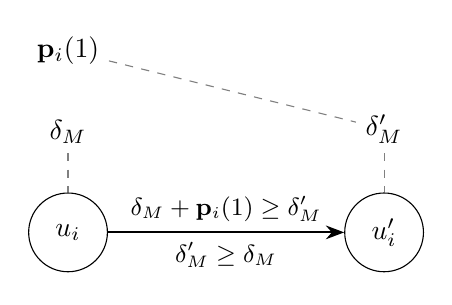
\begin{tikzpicture}[
    node distance=3cm,
    main node/.style={circle, draw, minimum size=1cm, inner sep=2pt},
    label/.style={font=\small, align=center},
    arrow/.style={-Stealth, thick}
]

% Nodes for u_i and u'_i
\node[main node] (ui) {$u_i$};
\node[main node, right=of ui] (ui') {$u'_i$};

% Inequality label between nodes
\draw[arrow] (ui) to node[label, above] {$\delta_M + \mathbf{p}_i(1) \geq \delta'_M$} 
                  node[label, below] {$\delta'_M \geq \delta_M$} (ui');

% Annotations for delta terms
\node[above=0.5cm of ui, anchor=south] (deltaM) {$\delta_M$};
\node[above=0.5cm of ui', anchor=south] (deltaM') {$\delta'_M$};
\node[above=1.5cm of ui, anchor=south] (p_i1) {$\mathbf{p}_i(1)$};

% Connect annotations to main nodes
\draw[dashed, gray] (deltaM) -- (ui);
\draw[dashed, gray] (deltaM') -- (ui');
\draw[dashed, gray] (p_i1) -- (deltaM');

\end{tikzpicture}
\end{document}